\achapter{9}{Sequences in Metric Spaces}\label{chap:sequences}

\vspace*{-17 pt}
\framebox{
\parbox{\dimexpr\linewidth-3\fboxsep-3\fboxrule}
{\begin{fqs}
\item What is a sequence in a metric space?
\item What does it mean for a sequence to have a limit in a metric space?
\item How can we use sequences to determine the continuity of a function at a point?
\end{fqs}}}

\vspace*{13 pt}

\csection{Introduction}\label{sec_seq_intro}

We were introduced to sequences in calculus, and we can extend the notion of the limit of a sequence to metric spaces. Sequences provide an alternate way to describe many ideas in metric space. For example, we will see that we can characterize continuity in terms of sequences, and we can use sequences to determine open and closed sets. 

Recall from calculus that a sequence of real numbers is a list of numbers in a specified order. We write a sequence $a_1$, $a_2$, $\ldots$, $a_n$, $\ldots$ as $(a_n)_{n \in \Z^+}$ or just $(a_n)$. If we think of each $a_n$ as the output of a function, we can give a more formal definition of a sequence as a function $f: \Z^+ \to \R$, where $a_n = f(n)$ for each $n$. 

A sequence $(a_n)$ of real numbers converges to a number $L$ if we can make all of the numbers in the sequence as close to $L$ as we like by choosing $n$ to be large enough. Once again, this is an informal description that we need to make more rigorous. As we saw with continuous functions, we can make more rigorous the idea of ``closeness" by introducing a symbol for a number that can be arbitrarily small. So we can say that the numbers $a_n$ can get as close to a number $L$ as we want if we can make $| a_n - L | < \epsilon$ for any positive number $\epsilon$. The idea of choosing $n$ large enough is just finding a large enough fixed integer $N$ so that $| a_n - L | < \epsilon$ whenever $n \geq N$. This leads to the definition.

\begin{definition} \label{def:sequence_limit_real} A sequence $(a_n)$ of real numbers has a \textbf{limit}\index{limit of a sequence of real numbers} $L$ if, given any $\epsilon > 0$ there exists a positive integer $N$ such that 
\[| a_n - L | < \epsilon \ \text{ whenever } \ n \geq N.\]
\end{definition}

When a sequence $(a_n)$ has a limit $L$, we write 
\[\lim_{n \to \infty} a_n = L,\]
or just $\lim a_n = L$ (since we assume the limit for a sequence occurs as $n$ goes to infinity) and we say that the sequence $(a_n)$ \emph{converges} to $L$.

\begin{example} We can draw a graph of a sequence $(a_n)$ of real numbers as the set of points $(n,a_n)$. In this way we can visualize a sequence and its limit. By definition, $L$ is a limit of the sequence $(a_n)$ if, given any $\epsilon > 0$, we can go far enough out in the sequence so that the numbers in the sequence all lie in the horizontal band between $y = L -\epsilon$ and $L+ \epsilon$ as illustrated in Figure \ref{F:sequence_limit} for the sequence $\left(\frac{n}{1+n}\right)$. 
\begin{figure}[h]
\begin{center}
\resizebox{!}{2.0in}{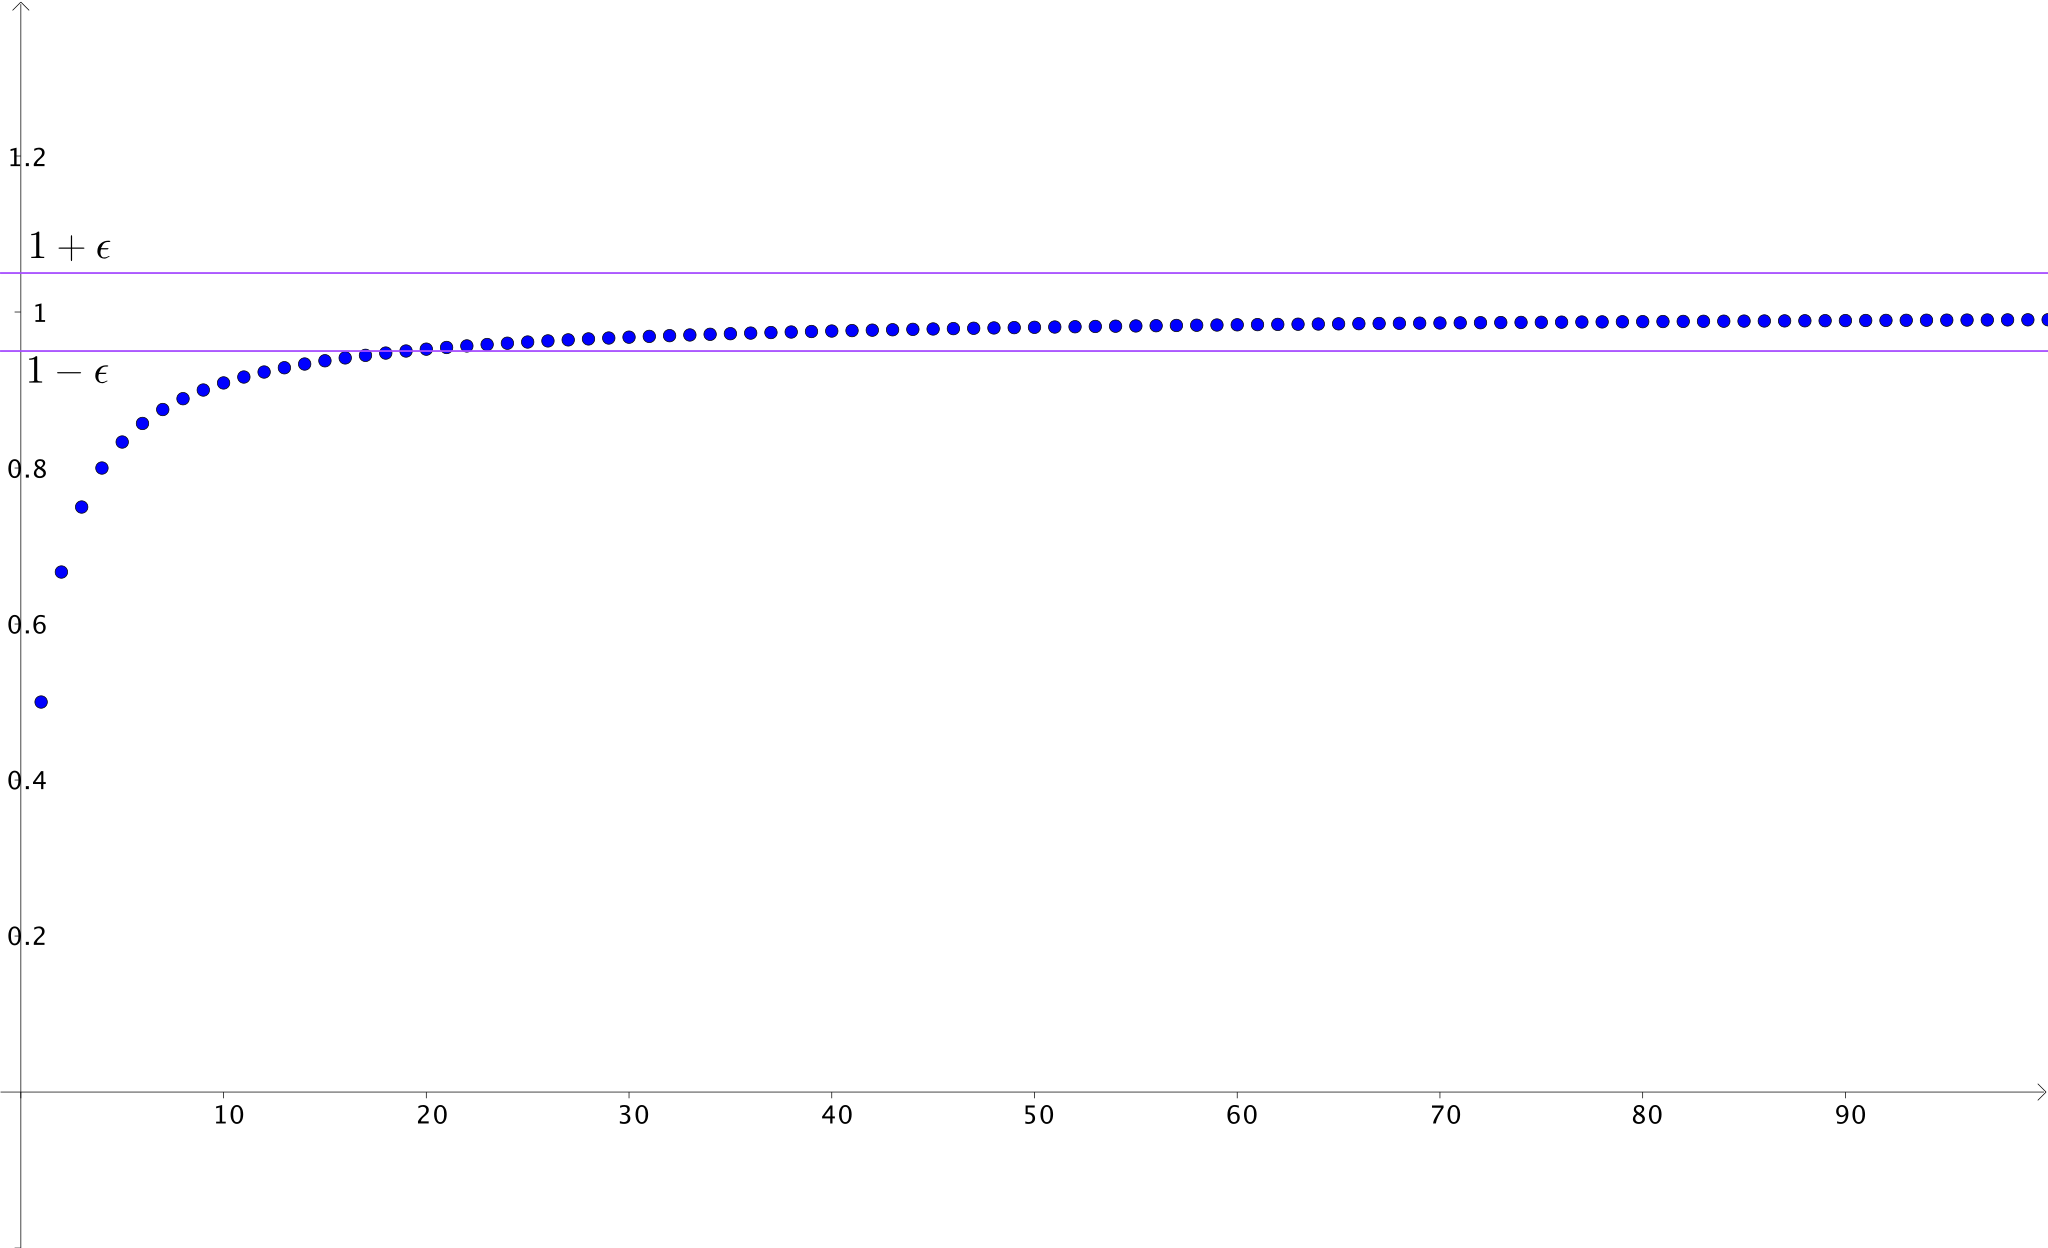
\includegraphics{Sequence_limit}}
\caption{The limit of the sequence $\left(\frac{n}{1+n}\right)$.} 
\label{F:sequence_limit}
\end{center}
\end{figure}
To verify that the limit of the sequence $\left(\frac{n}{1+n}\right)$ is $1$, we start with $\epsilon > 0$. 

\begin{quote} \textbf{Scratch work.} Now we need to find $N$ so that $n \geq N$ implies $\left| \frac{n}{1+n} - 1 \right| < \epsilon$. Just as with our continuity example, this work is not part of the proof, but shows how we go about finding the $N$ we need. To make $\left| \frac{n}{1+n} - 1 \right| < \epsilon$ we need
\begin{align*}
\left| \frac{n}{1+n} - 1 \right| &< \epsilon \\
\left| \frac{n}{1+n} - \frac{1+n}{1+n}  \right| &< \epsilon \\
\left| \frac{-1}{1+n} \right| &< \epsilon \\
1+n &> \frac{1}{\epsilon} \\
n &> \frac{1}{\epsilon} -1.
\end{align*}

Now we use this scratch work to design our proof. 
\end{quote}

Let $N > \frac{1}{\epsilon} -1$ (so that $N$ depends on $\epsilon$). Then for $n \geq N$ we have 
\begin{align*}
n &> N > \frac{1}{\epsilon} -1 \\
1+n &> \frac{1}{\epsilon} \\
|-1| \left| \frac{1}{1+n} \right| &< \epsilon \\
\left| \frac{-1}{1+n} \right| &< \epsilon \\
\left| \frac{n}{1+n} - 1 \right| &< \epsilon \\
\left| \frac{n}{1+n} - \frac{1+n}{1+n}  \right| &< \epsilon.
\end{align*}
So the sequence $\left(\frac{n}{1+n}\right)$ has a limit of $1$.
\end{example}

Definition \ref{def:sequence_limit_real} only applies to sequences of real numbers. Ultimately, we want to phrase the definition in a way that allows us to define limits of sequences in metric spaces and topological spaces. So we have to reformulate the definition in such a way that it does not depend on distances. 

Recall that $| x-y |$ defined a metric $d_E$ on $\R$, that is 
\[d_E(x,y) = | x-y |.\]
So we can rephrase the definition of a limit of a sequence of real numbers as follows.

\begin{definition}[Alternate Definition] A sequence $(a_n)$ of real numbers has a \textbf{limit} $L$ if, given any $\epsilon > 0$ there exists a positive integer $N$ such that 
\[d_E(a_n, L) < \epsilon \ \text{ whenever } \ n \geq N.\]
\end{definition}

Once we have described a limit of a sequence in terms of a metric, then we can extend the idea into any metric space. 

\begin{definition} A \textbf{sequence}\index{sequence in a metric space} in a metric space $(X,d)$ is a function $f: \Z^+ \to X$.  
\end{definition}

If $f$ is a sequence in $X$, we write the sequence defined by $f$ as $(f(n))$, where $n \in \Z^+$. We also use the notation $(a_n)$, when $a_n = f(n)$. As long as $X$ has a metric defined on it, we can then describe the limit of a sequence.

\begin{definition} Let $(X,d)$ be a metric space. A sequence $(a_n)$ in $X$ has a \textbf{limit}\index{limit of a sequence in a metric space} $L \in X$ if, given any $\epsilon > 0$ there exists a positive integer $N$ such that 
\[d(a_n, L) < \epsilon \ \text{ whenever } \ n \geq N.\]
\end{definition}

In other words, a sequence  $(a_n)$ in a metric space $(X,d)$ has a limit $L \in X$ if $\lim d(a_n,L) = 0$ -- or that the sequence $d(a_n,L)$ of real numbers has a limit of $0$. Just as with sequences of real numbers, when a sequence $(a_n)$ has a limit $L$, we say that the sequence $(a_n)$ \emph{converges} to $L$, or that $L$ is a limit of the sequence $(a_n)$. 

\begin{pa} ~
\be
\item Explain why the sequence $\left(\frac{1}{n}\right)$ converges to 0 in $\R$ using the Euclidean metric $d_E$, where 
\[d_E(a,y) = | x-y |.\]

\item Consider the sequence $(a_n) = \left(\left(\frac{1}{n}, \frac{1}{n+1} \right)\right)$ in $(\R^2, d_T)$, where $d_T$ is the taxicab metric
\[d_T((x_1, x_2), (y_1, y_1)) = | x_1-y_1| + | x_2-y_2 |.\]
Does the sequence $(a_n)$ converge? If so, find its limit and prove that your candidate is the limit. If not, explain why.

\item Let $(b_n) = \left((2n, n^2)\right)$ in the metric space $(\R^2, d)$, where $d$ is the discrete metric defined by 
\[d(x,y) = \begin{cases} 0 &\text{if } x=y \\ 1 &\text{if } x \neq y. \end{cases}\]
Does the sequence $(b_n)$ converge? If so, find its limit and prove that your candidate is the limit. If not, explain why.

\ee

\end{pa}


\begin{comment}

\ActivitySolution

\be
\item  Let $a_n = \frac{1}{n}$ for each positive integer $n$. Let $\epsilon > 0$. We will show that there is a positive integer $N$ such that $n \geq N$ implies $d_E(a_n,0) < \epsilon$. Since the set of positive integers is unbounded above, there exists a positive integer $N$ so that $\frac{1}{N} < \epsilon$. Then, if $n \geq N$, it follows that 
\[d_E(a_n,0) = | a_n-0 | = | \frac{1}{n} | \leq \frac{1}{N} < \epsilon.\]
We conclude that $lim \frac{1}{n} = 0$.   

\item  We will show that $\lim a_n = (0,0)$. Let $\epsilon > 0$. Choose $N \in \Z^+$ so that $N > \frac{2}{\epsilon}$. This makes $\frac{1}{N} < \frac{\epsilon}{2}$. Note that $\frac{1}{N+1} < \frac{1}{N} < \frac{\epsilon}{2}$ as well. Now let $n \geq N$. Then 
\begin{align*}
d_T(a_n, (0,0)) &= \left| \frac{1}{n} - 0 \right| + \left| \frac{1}{n+1} - 0 \right| \\
	&= \frac{1}{n} + \frac{1}{n+1} \\
	&\leq \frac{1}{N} + \frac{1}{N+1} \\
	&< \frac{\epsilon}{2} + \frac{\epsilon}{2} \\
	&= \epsilon.
\end{align*}


\item  We claim that the sequence $(b_n)$ does not have a limit. To demonstrate this, we proceed by contradiction and assume that the sequence $(b_n)$ has a limit $b$. So for any $\epsilon > 0$ there exists an integer $N > 0$ so that $n \geq N$ implies $d(b_n,b) < \epsilon$. Let $\epsilon = \frac{1}{2}$. Now $(2n,n^2) \neq (2m,m^2)$ if $m \neq n$ in $\Z$, so all of the entries of the sequence $(b_n)$ are distinct. Now either $b = b_n$ for some $n$ or $b \neq b_n$ for all $n$. In either case there is a large enough $N$ so that $b \neq b_n$ for all $n \geq N$. Then $n \geq N$ implies 
\[d(b_n,b) = 1 > \epsilon.\]
So there cannot be an integer $N > 0$ so that $d(b_n,b) < \epsilon$ for $n \geq N$, no matter what $b$ is, so the sequence $(b_n)$ does not have a limit.

\ee

\end{comment}

\csection{Sequences and Continuity in Metric Spaces}\label{sec_seq_cont_metric}

There are different characterizations of continuity. We have already see the $\epsilon$-$\delta$ definition and a characterization in terms of neighborhoods. In this section we investigate sequences and limits of sequences in metric spaces, and then provide a characterization of continuous functions in terms of sequences. 

\begin{activity} A reasonable question to ask is if a limit of a sequence is unique. We will answer that question in this activity. Let $(X,d)$ be a metric space and $(a_n)$ a sequence in $X$. Assume the sequence $(a_n)$ has a limit in $X$. To show that a limit of the sequence $(a_n)$ is unique, we need to show that if $\lim a_n = a$ and $\lim a_n = a'$ for some $a, a' \in X$, then $a=a'$.

Suppose $\lim a_n = a$ and $\lim a_n = a'$ for some $a, a' \in X$. Without much to go on it might appear that proving $a=a'$ is a difficult task. However, if $d(a,a') < \epsilon$ for any $\epsilon > 0$, then it will have to be the case that $a=a'$. So let $\epsilon > 0$. 

	\ba
	\item Why must there exist a positive integer $N$ so that $d(a_n, a) < \frac{\epsilon}{2}$ for all $n \geq N$?

	\item Why must there exist a positive integer $N'$ so that $d(a_n, a') < \frac{\epsilon}{2}$ for all $n \geq N'$?

	\item Now let $m = \max\{N, N'\}$. What can we say about $d(a_m,a)$ and $d(a_m,a')$? Why?
	
	\item Use the triangle inequality to conclude that $d(a,a') < \epsilon$. What else can we conclude?

	\ea

\end{activity}

\begin{comment}

\ActivitySolution
	\ba
	\item Since $a$ is a limit of $(a_n)$, the definition of a limit of a sequence states that, given $\frac{\epsilon}{2}$ (using $\frac{\epsilon}{2}$ in place of $\epsilon$), there exists a positive integer $N$ so that $d(a_n, a) < \frac{\epsilon}{2}$ for all $n \geq N$.

	\item Since $a'$ is a limit of $(a_n)$, the definition of a limit of a sequence states that, given $\frac{\epsilon}{2}$ (using $\frac{\epsilon}{2}$ in place of $\epsilon$), there exists a positive integer $N'$ so that $d(a_n, a') < \frac{\epsilon}{2}$ for all $n \geq N'$.

	\item Since $m$ is larger than $N$ we know that $d(a_m,a) < \frac{\epsilon}{2}$. Since $m$ is larger than $N'$ we know that $d(a_m,a') < \frac{\epsilon}{2}$. 
		
	\item We now have that
	\[d(a,a') \leq d(a,a_m) + d(a_m,a') < \frac{\epsilon}{2} + \frac{\epsilon}{2} = \epsilon.\]
	From this we can conclude that $a = a'$. 
	
	\ea

\end{comment}

Continuity can also be described in terms of sequences. The basic idea is this. Suppose that $f : \R \to \R$ is continuous at a point $a$. This means that $f$ has a limit (as a continuous function) at $a$. So if we were to take any sequence $(a_n)$ that converges to $a$, then the continuity of $f$ implies that $f(a) = f(\lim a_n) = \lim f(a_n)$. That this is both a necessary condition and a sufficient condition for continuity is given in the next theorem.

\begin{theorem} \label{thm:seq_continuity}  Let $(X,d_X)$ and $(Y,d_Y)$ be metric spaces, and let $a \in X$. A function $f:X \to Y$ is continuous at $a$ if and only if $\lim f(a_n) = f(a)$ for any sequence $(a_n)$ in $X$ that converges to $a$. 
\end{theorem}

\begin{proof} Let $(X,d_X)$ and $(Y,d_Y)$ be metric spaces, let $a \in X$, and let $f: X \to Y$ be a function. Assume that $f$ is continuous at $a$. We will show that $\lim f(a_n) = f(a)$ for any sequence $(a_n)$ in $X$ that converges to $a$. Let $(a_n)$ be a sequence in $X$ that converges to $a$ (we know such a sequence exists, namely the sequence $(a)$). To verify that $\lim f(a_n) = a$, let $\epsilon > 0$. The fact that $f$ is continuous at $a$ means that there is a $\delta > 0$ so that $d_Y(f(x), f(a)) < \epsilon$ whenever $d_X(x,a) < \delta$. Since $(a_n)$ converges to $a$, we know that there exists a positive integer $N$ such that $d_X(a_n, a) < \delta$ whenever $n \geq N$. This implies that 
\[d_Y(f(a_n), f(a)) < \epsilon \ \text{ whenever } \ n \geq N.\]
We conclude that if $f$ is continuous at $a$, then $\lim f(a_n) = f(a)$ for any sequence $(a_n)$ in $X$ that converges to $a$.

The proof of the reverse implication is contained in the next activity.
\end{proof}


\begin{activity} Let $(X,d_X)$ and $(Y,d_Y)$ be metric spaces, let $a \in X$, and let $f: X \to Y$ be a function. We prove the remaining implication of Theorem \ref{thm:seq_continuity}, that $f$ is continuous at $a$ if $\lim f(a_n) = f(a)$ for any sequence $(a_n)$ in $X$ that converges to $a$, in this activity. 
\ba
\item To have an additional assumption with which to work, let us proceed by contradiction and assume that $f$ is not continuous at $a$. Why can we then say that there is an $\epsilon > 0$ so that there is no $\delta > 0$ with the property that $d_X(x,a) < \delta$ implies $d_Y(f(x), f(a)) < \epsilon$?

\item To create a contradiction, we will construct a sequence $(a_n)$ that converges to $a$ while $(f(a_n))$ does not converge to $f(a)$. 
	\begin{enumerate}[i.]
	\item Explain why we can find a positive integer $K$ such that $\frac{1}{K} < \epsilon$.
	
	\item If $k > K$, explain why there is an element $a_k \in B\left(a, \frac{1}{k}\right)$ so that $d_Y(f(a_k), f(a)) \geq \epsilon$.

\item For $k \leq K$, let $a_k$ be any element in $B\left(a, \frac{1}{k}\right)$. Explain why $a$ is a limit of $(a_n)$. 

\item Explain why $f(a)$ is not a limit of the sequence $(f(a_n))$. What conclusion can we draw, and why? 

	\end{enumerate}
\ea

\end{activity}

\begin{comment}

\ActivitySolution

\ba
\item Since $f$ is not continuous at $a$, we negate the definition of continuity, negating universal and existential quantifiers. This tells us that exists an $\epsilon > 0$ such that there is no $\delta > 0$ with the property that $d_X(x,a) < \delta$ implies $d_Y(f(x), f(a)) < \epsilon$.

\item 
	\begin{enumerate}[i.]
	\item The sequence $\frac{1}{k}$ of real numbers converges to $0$, so we can make $\frac{1}{k}$ as close to $0$ as we like. That means we can make $\frac{1}{k}$ less than $\epsilon$ if $k$ is large enough. So there is some positive integer $K$ such that $\frac{1}{K} < \epsilon$. 
	
	\item From part (a), for each $k > K$ there is no $\delta$  with the property that $d_X(x,a) < \delta$ implies $d_Y(f(x), f(a)) < \epsilon$. Thus, there must be some element $a_k$ with $d_X(a_k,a) < \frac{1}{k}$ and $d_Y(f(a_k),f(a)) > \epsilon$. Since $d_X(a_k,a) < \frac{1}{k}$, we know that $a_k \in B\left(a, \frac{1}{k}\right)$. 
	
	\item Choosing any $a_k \in B\left(a, \frac{1}{k}\right)$ when $k \leq K$ gives us a sequence $(a_n)$. We now show that $a$ is the limit of $(a_n)$. Let $\alpha > 0$. Let $N$ be a positive integer such that $\frac{1}{N} < \alpha$. If $n \geq N$, since $a_n \in B\left(a, \frac{1}{n}\right)$, we see that 
	\[d_X(a_n,a) < \frac{1}{n} < \frac{1}{N} < \alpha.\]
	Therefore, the sequence $(a_n)$ has a limit of $a$. 
	
	\item  Now we demonstrate that $(f(a_n))$ does not have $f(a)$ as a limit. Using $\epsilon$ as given, note that $n > K$ implies that $d_Y(f(a_k), f(a)) \geq \epsilon$. We can always choose $n$ larger enough so that $\frac{1}{n} < \delta$ for any given $\delta > 0$. So there can be no $\delta$ such that $d(x,a) < \delta$ implies $d_Y(f(a_k),f(a)) < \epsilon$. 

	\item Assuming that $f$ is not continuous at $a$ led to the construction of a sequence $(a_n)$ with limit $a$, but $\lim f(a_n) \neq f(a)$. This contradicts our hypothesis. We must therefore conclude that $f$ is continuous at $a$. 

	\end{enumerate}
\ea


\end{comment}

One way that Theorem \ref{thm:seq_continuity} is often used is illustrated in the next activity. 

\begin{activity} \label{act:sequence_continuity} Let $f$ be the function from $\R$ to $\R$, both with the Euclidean metric, defined by 
\[f(x) = \begin{cases} \sin\left(\frac{1}{x}\right) &\text{ if } x \neq 0 \\ 0 &\text{ if } x = 0. \end{cases}\]
We consider the $f$ continuity of $f$ at $0$ in this activity.

	\ba
	\item Draw a graph of $f$ on some small interval centered at $0$. Based on the  graph, do you think $f$ has a limit at $0$? Explain. (There is no right answer here, just your intuition based on the graph.)
	
	\item At which inputs is $f(x)=1$? 
	
	\item Use the result of (b) to find a sequence $(a_n)$ that converges to $0$ for which $f(a_n) = 1$ for every $n$.
	
	\item What does the result of (c) tell us about the continuity of $f$ at $0$? 
	

	\ea

\end{activity}

\begin{comment}

\ActivitySolution

\ba

\item A graph of $f$ on the interval $[-1,1]$ is shown in Figure \ref{F:top_sine}. Based on the appearance of the graph, it looks as though the graph oscillates back and forth infinitely often between $-1$ and $1$ as $x$ gets close to $0$. So we don't expect the function $f$ to have a limit at $0$.  
\begin{figure}[h]
\begin{center}
\resizebox{!}{2.0in}{\includegraphics{topologist_sine}}
\caption{A graph of $f(x)$.} 
\label{F:top_sine}
\end{center}
\end{figure}

\item We will have $f(x) = 1$ when $\sin\left(\frac{1}{x}\right) = 1$. This happens when $\frac{1}{x} = \frac{\pi}{2} + k \pi$ for any integer $k$, or when 
\[x = \frac{1}{\frac{\pi}{2} + k \pi}.\]

\item Let $a_n = \frac{1}{\frac{\pi}{2} + n \pi}$. As $n$ goes to infinity, $a_n$ converges to $0$. But $f(a_n) = 1$ for every $n$. This means that if $f$ has a limit at $0$, that limit has to be $1$. But $f(0) = 0$, so $f$ is not continuous at $0$. 

\ea

\end{comment}

While it can sometimes be difficult to prove a fact about all sequences that converge to a point, Activity \ref{act:sequence_continuity} shows that we can use Theorem \ref{thm:seq_continuity} to prove that a function $f$ is not continuous at an input $a$ be finding just one sequence $(a_n)$ that converges to $a$ for which $\lim f(a_n) \neq f(a)$. We conclude this section with one final note. 

\noindent IMPORTANT NOTE: Theorem \ref{thm:seq_continuity} tells us that if $f : X \to Y$ is a continuous function, then $f$ commutes with limits. That is, if $(a_n)$ is a sequence in $X$ that converges to $a \in X$, then 
\[f(a) = f(\lim a_n) = \lim f(a_n).\]


 \csection{Summary}\label{sec_seq_summ}
Important ideas that we discussed in this section include the following.
\begin{itemize}
\item A sequence in a metric space $X$ is a function $f : \Z^+ \to X$.
\item  A sequence $(a_n)$ in a metric space $(X,d)$ has a limit $L$ in $X$ if, given any $\epsilon > 0$ there exists a positive integer $N$ such that $d(a_n,L) < \epsilon$ whenever $n \geq N$.
\item Let $f$ be a function from a metric space $(X,d_X)$ to m metric space $(Y,d_Y)$. Then $f$ is continuous at $a \in X$ if and only if $\lim f(a_n) = f(a)$ for any sequence $(a_n)$ in $X$ that converges to $a$.
\end{itemize}

\csection{Exercises}\label{sec_seq_exer}

\be

\item Determine, with proof, the convergence or divergence of each of the following sequences in the indicated metric spaces.

\ba

\item $a_n = 1+\frac{1}{n}$ in $(\R, d_E)$

\item $a_n = (2,n)$ in $(\R^2, d_M)$

\item $a_n$ is the function defined by 
\[a_n(x) = \frac{1}{n}x\]
where $X$ is the set of real valued functions on the interval $[0,1]$ and the metric $d$ is defined by 
\[d(f,g) = \sup\{|f(x)-g(x)| \mid x \in [0,1]\}.\]
(See Exercise \ref{ex:GLB_function_sup_metric} on page \pageref{ex:GLB_function_sup_metric}.)


\ea

\begin{comment}

\ExerciseSolution 

\ba

\item We prove that $(a_n)$ converges to $1$. Let $\epsilon$ be a positive real number. We know there is an $N \in \Z^+$ such that $\frac{1}{N} < \epsilon$. Then if $n \geq N$, 
\[|a_n - 1| = \left|\frac{1}{n}\right| < \frac{1}{N} < \epsilon.\]
Therefore, $\lim a_n = 1$. 

\item We prove that $(a_n)$ has no limit. Let $a = (u,v)$ be a point in $\R^2$ and let $\epsilon$ be a positive real number.  We know that 
\[d_M(a_n,a) = \max\{|2-u|, |n-v|\}.\]
By the Archimedean property, there is $M \in \Z^+$ such that $M - v \geq \epsilon$. So if $n \geq M$ we have 
\[d_M(a_n,a) = \max\{|2-u|, |n-v|\} \geq |n-v| > M-v \geq \epsilon.\] 
So there can be no $N \in \Z^+$ with $d_M(a_n,a) < \epsilon$ whenever $n \geq N$. We conclude that the sequence $(a_n)$ has no limit. 

\item We prove that the sequence $(a_n)$ converges to the constant function $a$ defined by $a(x) = 0$ for all $x \in [0,1]$. Notice that $a_n(x)$ is the linear function connecting the points $(0,0)$ and $\left(1,\frac{1}{n}\right)$. So 
\[d(a_n,a) = \sup\{|a_n(x)-a(x)| \mid x \in [0,1]\} = \left(\frac{1}{n}-0\right| = \frac{1}{n}.\]
Let $\epsilon > 0$. By the Archimedean property, there is an $N \in \Z^+$ such that $N > \frac{1}{\epsilon}$. Then for $n \geq N$ we have 
\[d(a_n,a) = \frac{1}{n} \leq \frac{1}{N} < \epsilon.\]

\ea

\end{comment}


\item Let $A$ be a subset of $\R$.

\ba

\item Show that if $A$ is bounded above, then there is a sequence $(a_n)$ in $A$ such that $\lim a_n = \sup(A)$. 

\item Show that if $A$ is bounded below, then there is a sequence $(a_n)$ in $A$ such that $\lim a_n = \inf(A)$. 

\item Are the limits from (a) or (b) necessarily in $A$? Explain.
\ea

\begin{comment}

\ExerciseSolution

\ba

\item Assume that $A$ is bounded above so that $s = \sup(A)$ exists. Let $n \in \Z^+$. Since $s-\frac{1}{n} < s$, we know that $s-\frac{1}{n}$ is not an upper bound for $A$. So there exists $a_n \in A$ such that $s-\frac{1}{n} < a_n \leq s$. Given any $\epsilon > 0$, there exists $N \in \Z^+$ such that $\frac{1}{N} < \epsilon$. So if $n \geq N$, then $|a_n - s| < \frac{1}{n} < \frac{1}{N} < \epsilon$. We conclude that $\lim a_n = s$. 

\item Assume that $A$ is bounded above so that $t = \inf(A)$ exists. Let $n \in \Z^+$. Since $t+\frac{1}{n} < t$, we know that $t+\frac{1}{n}$ is not a lower bound for $A$. So there exists $a_n \in A$ such that $t \leq a_n < t+\frac{1}{n}$. Given any $\epsilon > 0$, there exists $N \in \Z^+$ such that $\frac{1}{N} < \epsilon$. So if $n \geq N$, then $|a_n - t| < \frac{1}{n} < \frac{1}{N} < \epsilon$. We conclude that $\lim a_n = t$. 

\item Let $A$ be the open interval $(0,1)$ in $\R$ with the Euclidean metric.  Then $\sup(A) = 1$ and $\inf(A) = 0$. So neither limit needs to be in $A$.  
\ea

\end{comment}

\item Let $(X,d)$ be a metric space, let $x \in X$, and let $A$ be a nonempty subset of $X$. Recall that the distance from $x$ to $A$ is 
\[d(x,A) = \inf \{d(x,a) \mid a \in A.\]
In this exercise we see how we can view the distance between a point and a set in terms of sequences. Let $m = d(x,A)$. We will show that there must be a sequence $(a_n)$ in $A$ so that $d(x,A) = \lim d(x,a_n)$. 
\ba
\item For each $n \in \Z^+$, let $B_n = B\left(x;m+\frac{1}{n}\right)$. Why must $B_n \cap A \neq \emptyset$ for each $n \in \Z^+$? 

\item Let $a_n \in B_n \cap A$ for each $n$. What property does this sequence have? Explain how we have just proved the following theorem.

\begin{theorem} Let $(X,d)$ be a metric space, let $x \in X$, and let $A$ be a nonempty subset of $X$. Then there exists a sequence $(a_n)$ in $A$ such that 
\[\lim d(x,a_n) = d(x,A).\]
\end{theorem}

\ea


\begin{comment}

\ExerciseSolution

\ba
\item Suppose to the contrary that there is an $n \in \Z^+$ such that $B_n \cap A = \emptyset$. Then there is no element $c \in A$ such that $d(x,c) < m + \frac{1}{n}$. This makes $m + \frac{1}{n}$ a lower bound for $\{d(x,a) \mid a \in A\}$ greater than the greatest lower bound of $\{d(x,a) \mid a \in A\}$. Since this cannot happen, we conclude that $B_n \cap A \neq \emptyset$ for every $n \in \Z^+$. 

\item We have
\[\lim d(x,a_n) \leq \lim \left(m+\frac{1}{n}\right) = m.\]
So we have found a sequence $(a_n)$ in $A$ satisfying $\lim d(x,a_n) = d(x,A)$.

\ea

\end{comment}

\item ~
	\ba
	\item Let $(Y,d')$ be a subspace of $(X,d)$. Let $a_1$, $a_2$, $\ldots$ be a sequence of points in $Y$ and let $a \in Y$. Prove that if $\lim_n a_n = a$ in $(Y,d')$, then $\lim_n a_n = a$ in $(X,d)$. 

	\item Show that the converse of part (a) is false by considering the subspace $(\Q, d_{\Q})$ (the rational numbers) of $(R,d)$. Let $a_1$, $a_2$, $\ldots$ be a sequence of rational numbers such that $\lim_n a_n = \sqrt{2}$. Prove that , given $\epsilon > 0$, there is a positive integer $N$ such that for $n, m > N$, $|a_n - a_m | < \epsilon$. Does the sequence  $a_1$, $a_2$, $\ldots$ converge when considered to be a sequence of points in $\Q$?  

	\ea

\begin{comment}

\ExerciseSolution 
\ba
\item Let $(Y,d')$ be a subspace of $(X,d)$. Let $a_1$, $a_2$, $\ldots$ be a sequence of points in $Y$ and assume $\lim_n a_n = a$ for some $a \in Y$. Let $\epsilon > 0$. Then there exists an $N \in \Z^+$ so that $d'(a_n,a) < \epsilon$ whenever $n \geq N$. But $d'(a_n,a) = d(a_n,a)$, so $d(a_n,a) < \epsilon$ whenever $n \geq N$. This implies that $\lim a_n = a$ in $X$. 

\item Here we assume $d = d_E$ in $\R$ and that $d_{\Q}$ is the restriction of $d$ to $\Q$. Let $\epsilon > 0$. Since $\lim a_n = \sqrt{2}$, there exists $N \in \Z^+$ so that $n \geq N$ implies $| a_n - \sqrt{2} | < \frac{\epsilon}{2}$. Now let $n, m > N$. The triangle inequality then gives us \[| a_n - a_m | \leq | a_n - \sqrt(2)| + | \sqrt{2} - a_m | < \frac{\epsilon}{2} + \frac{\epsilon}{2} = \epsilon.\]

Now we will show that the sequence $(a_n)$ does not converge as a sequence in $\Q$. Assume to the contrary that the sequence $(a_n)$ does converge as a sequence in $\Q$. The uniqueness of limits then implies that $\sqrt{2}$ is a rational number. That means that $\sqrt{2} = \frac{p}{q}$ for some relatively prime positive integers $p$ and $q$. This implies that $q\sqrt{2} = p$ or $2q^2 = p^2$. The fact that $2$ divides $p^2$ means that $p$ must be even. So $p = 2r$ for some positive integer $r$. It follows that 
\[2q^2 = (2r)^2 = 4r^2.\]
But then $q^2 = 2r^2$ and $2$ divides $q$. This contradicts the fact that $p$ and $q$ are relatively prime. So $\sqrt{2}$ is not a rational number and the sequence $(a_n)$ does not converge as a sequence in $\Q$.  

\ea

\end{comment}

\item \label{ex:limit_properties} In this exercise we prove some standard results about limits of sequences from calculus. Let $(a_n)$ and $(b_n)$ be convergent sequences in a metric space $(\R,d_E)$. 

\ba

\item Show that $\lim ka_n = k \lim a_n$ for any real number $k$.

\item Show that $\lim (a_n + b_n) = \lim a_n + \lim b_n$. 

\item Show that the sequence $(a_n)$ is bounded. That is, show that there is a positive real number $M$ such that $|a_n| \leq M$ for all $n \in \Z^+$. 

\item Show that $\lim a_nb_n = \lim a_n \ \lim b_n$. 

\item If $b_n \neq 0$ for every $n$ and $\lim b_n \neq 0$, show that $\lim \frac{a_n}{b_n} = \frac{\lim a_n}{\lim b_n}$. 

\ea

\begin{comment}

\ExerciseSolution

\ba

\item Let $a = \lim a_n$, let $k \in \R$, and let $\epsilon$ be a positive real number. If $k = 0$, then 
\[\lim ka_n = \lim 0 = 0 = 0(a) = 0\lim a_n.\]
So suppose $k \neq 0$. Let $N \in \Z^+$ such that $d(a_n, a) < \frac{\epsilon}{|k|}$ if $n \geq N$. So if $n \geq N$, then 
\[d_E(ka_n, ka) = |k|d_E(a_n,a) < |k| \frac{\epsilon}{|k|} = \epsilon.\]
So $\lim ka_n = ka$. 

\item Let $a = \lim a_n$, $b = \lim b_n$, and let $\epsilon$ be a positive real number. There exists $N_1 \in \Z^+$ such that $d_E(a_n,a) < \frac{\epsilon}{2}$ whenever $n \geq N_1$, and there exists $N_2 \in \Z^+$ such that $d_E(b_n,b) < \frac{\epsilon}{2}$ whenever $n \geq N_2$. Let $N = \max\{N_1, N_2\}$. Then if $n \geq N$ we have 
\begin{align*}
d_E(a_n+b_n, a+b) &= |(a_n+b_n) - (a+b)| \\
	&= |(a_n-a) + (b_n-b)| \\
	&\leq |a_n-a| + |b_n-b| \\
	&< \frac{\epsilon}{2} + \frac{\epsilon}{2} \\
	&= \epsilon.
\end{align*}
Therefore,  $\lim (a_n + b_n) = \lim a_n + \lim b_n$. 

\item Let $a = \lim a_n$. There exists $N \in \Z^+$ such that $d_E(a_n,a) < 1$ whenever $n \geq N$. Thus, if $n \geq N$, we have $|a_n-a| < 1$ or $a-1 < a_n < a+1$. So $|a_n| < K$ for $n \geq N$, where $K = \max\{|a-1|, |a+1|\}$. Let $M = \max\{|a_1|, |a_2|, \ldots, |a_{N-1}|, K\}$. Then $|a_n| \leq M$ for all $n \in \Z^+$. 
 
\item Let $a = \lim a_n$, $b = \lim b_n$, and let $\epsilon$ be a positive real number. The sequence $(b_n)$ is bounded by the previous part of this problem, so let $M$ be an upper bound for $\{|b_n| \mid n \in \Z^+\}$. There exists $N_1 \in \Z^+$ such that $d_E(a_n,a) < \frac{\epsilon}{2(K+1)}$ whenever $n \geq N_1$, and there exists $N_2 \in \Z^+$ such that $d_E(b_n,b) < \frac{\epsilon}{2(|a|+1)}$ whenever $n \geq N_2$. Let $N = \max\{N_1, N_2\}$. Then if $n \geq N$ we have 
\begin{align*}
d_E(a_nb_n, ab) &= |a_nb_n - ab| \\
	&= |a_nb_n - b_na + b_na- ab| \\
	&= |b_n(a_n-a) + a(b_n-b)| \\
	&\leq |b_n| |a_n-a| + |a| |b_n-b| \\
	&< K\left(\frac{\epsilon}{2(K+1)} + |a|\frac{\epsilon}{2(|a|+1)}\right) \\
	&< \frac{\epsilon}{2} + \frac{\epsilon}{2} \\
	&= \epsilon.
\end{align*}
Therefore,  $\lim (a_nb_n) = \lim a_n \ \lim b_n$. 


\item Let $b = \lim b_n$. If we show that $\lim \frac{1}{b_n} = \frac{1}{\lim b_n}$, then we can use the result of the previous part because
\[\lim \frac{a_n}{b_n} = \lim a_n \ \lim \frac{1}{b_n} = \lim a_n \ \frac{1}{\lim b_n} = \frac{\lim a_n}{\lim b_n}.\]

One result we will need is that the sequence $(b_n)$ is bounded below by a positive number. There is an $N \in \Z^+$ such that $|b_n - b| < \frac{|b|}{2}$ whenever $n \geq N$. So if $n \geq N$, then $|b_n| > \frac{|b|}{2}$. Let $M = \min\left\{|a_1|, |a_2|, \ldots, |a_{N-1}|, \frac{|b|}{2}\right\}$. Then $|a_n| \geq M$ for all $n \in \Z^+$. 

Now let $\epsilon$ be a positive number. Let $M > 0$ be a lower bound for the sequence $(b_n)$. There exists $N \in \Z^+$ such that $d_E(b_n,b) < \epsilon \ |b| \ M$ whenever $n \geq N$. So if $n \geq N$, then 
\begin{align*}
d_E\left(\frac{1}{b_n}, \frac{1}{b}\right) &= \left| \frac{1}{b_n} - \frac{1}{b} \right| \\
	&= \left| \frac{b-b_n}{bb_n} \right| \\
	&\leq \frac{1}{|bb_n|} \epsilon \ |b| \ M \\
	&= \frac{M}{|b_n|} \epsilon \\
	&< \epsilon.
\end{align*}
So $\lim \frac{1}{b_n} = \frac{1}{\lim b_n}$ as desired.
	

\ea

\end{comment}


\item Let $f$ and $g$ be continuous functions from $\R$ to $\R$, both with the standard Euclidean metric. Define the function $fg$ from $\R$ to $\R$ by 
\[(fg)(x) = f(x)g(x) \text{ for every } x \in \R.\]
	\ba
	\item Prove that $fg$ is a continuous function.
	
	\item Assume that $g(x) \neq 0$ for every $x \in \R$. Define the function $\frac{f}{g}$ from $\R$ to $\R$ by $\frac{f}{g}(x) = \frac{f(x)}{g(x)}$ for every $x \in \R$. Use the definition of continuity to prove that $\frac{f}{g}$ is a continuous function.
	
	\ea
	
\begin{comment}

\ExerciseSolution

\ba
\item Let $a \in \R$. Let $(a_n)$ be a sequence in $\R$ that converges to $a$. Since $f$ and $g$ are continuous at $a$, we know that $\lim f(a_n) = f(a)$ and $\lim g(a_n) = g(a)$. We use the result of Exercise \ref{ex:limit_properties} on the sequences $(f(a_n))$ and $(g(a_n))$. to see that 
\[\lim (fg)(a_n) = \lim f(a_n)g(a_n) = \lim f(a_n) \lim g(a_n) = f(a) g(a).\]
So $fg$ is continuous at $a$. 

\item Similar to part (a) we have 
\[\lim \left(\frac{f}{g}\right)(a_n) = \lim \frac{f(a_n)}{g(a_n)} = \frac{\lim f(a_n)}{ \lim g(a_n)} = \frac{f(a)}{g(a)}.\]
So $\frac{f}{g}$ is continuous at $a$. 

\ea

\end{comment}

\item Let $(c_n) = (a_n,b_n)$ be a sequence in $(\R^2, d_E)$. Show that the sequence $(c_n)$ converges to a point $(a,b)$ if and only if $(a_n)$ converges to $a$ and $(b_n)$ converges to $b$ in $(\R, d_E)$. 

\begin{comment}

\ExerciseSolution First assume that the sequence $(c_n)$ converges to a point $c = (a,b) \in \R^2$. Let $\epsilon$ be a positive number. There exists $N \in \Z^+$ such that $d_E(c_n, c) < \epsilon$ whenever $n \geq N$. So if $n \geq N$ we have
\begin{align*}
d_E(a_n, a) &= |a_n-a| \\
	&\leq \sqrt{ |a_n-a|^2 + |b_n-b|^2} \\
	&= d_E(c_n,c) \\
	&< \epsilon
\end{align*}
and 
\begin{align*}
d_E(b_n, b) &= |b_n-b| \\
	&\leq \sqrt{ |a_n-a|^2 + |b_n-b|^2} \\
	&= d_E(c_n,c) \\
	&< \epsilon.
\end{align*}
We conclude that $(a_n)$ converges to $a$ and $(b_n)$ converges to $b$.

For the converse, we will use the following result:

\begin{lemma} Let $x$ and $y$ be real numbers. Then 
\[\sqrt{x^2+y^2} \leq |x| + |y|.\]
\end{lemma}

\begin{proof} Let $x$ and $y$ be real numbers. Then 
\begin{align*}
x^2 + y^2 &\leq |x|^2 + 2|x| \ |y| + |y|^2 \\
x^2 + y^2 &\leq (|x|+|y|)^2 \\
\sqrt{x^2+y^2} \leq |x| + |y|.
\end{align*}
\end{proof}

Now assume that $(a_n)$ converges to $a$ and $(b_n)$ converges to $b$ in $(\R, d_E)$. Let $c = (a,b)$ and let $\epsilon$ be a positive real number. There exists $N_1 \in \Z^+$ such that $d_E(a_n,a) < \frac{\epsilon}{2} $ whenever $n \geq N_1$ and there exists $N_2 \in \Z^+$ such that $d_E(b_n,b) < \frac{\epsilon}{2} $ whenever $n \geq N_2$. Let $N = \max\{N_1, N_2\}$. Then, using the lemma, if $n \geq N$ we have
\begin{align*}
d_E(c_n,c) &= \sqrt{ |a_n-a|^2 + |b_n-b|^2} \\
	&\leq |a_n-a| + |b_n-b| \\
	&= d_E(a_n,a) + d_E(b_n,b) \\
	&< \frac{\epsilon}{2} + \frac{\epsilon}{2} \\
	&= \epsilon.
\end{align*}
We conclude that $(c_n)$ converges to $c$ in $(\R^2, d_E)$. 

\end{comment}

\item Define $f : (\R,d_E) \to (\R,d_E)$ by 
\[f(x) = \begin{cases} 0 &\text{ if } x \text{ is irrational} \\ x &\text{ if } x \text{ is rational.} \end{cases}\]

\ba

\item Show that $f$ is continuous at exactly one point. Assume that both copies of $\R$ are given the Euclidean topology.

\item Modify the function $f$ to construct a new function $g: \R \to \R$ such that $g$ is continuous at exactly the numbers $0$ and $1$. Prove your result. Can you see how to extend this to construct a function $h: \R \to \R$ that is continuous at any given finite number of points? 

\ea

\begin{comment}

\ExerciseSolution 

\ba

\item First we demonstrate that $f$ is not continuous at every nonzero input. Suppose $a \neq 0$. Every ball centered at $a$ contains a rational number and an irrational number. So for each $n \in \Z^+$, there is a rational number $r_n$ and an irrational number $i_n$ in $B\left(a,\frac{1}{n}\right)$. But then $r_n \to a$ and $i_n \to a$. If $f$ were continuous at $a$, then $f(r_n) \to f(a)$ and $f(i_n) \to f(a)$. But $f(r_n) = r_n \to a$ while $f(i_n) = 0 \to 0 \neq a$. Thus, $f$ is not continuous at $a$. 

Now we demonstrate that $f$ is continuous at $0$. Let $(s_n)$ be a sequence of real numbers with $s_n \to 0$.  Note that $|f(s_n)| \leq |s_n|$, so the fact that $s_n \to 0$ implies that $f(s_n) \to 0$. Therefore, $f$ is continuous at $0$.

\item Define $g: \R \to \R$ by 
\[g(x) = \begin{cases} 0 &\text{ if } x \text{ is irrational} \\ x(x-1) &\text{ if } x \text{ is rational.} \end{cases}\]

First we demonstrate that $g$ is not continuous at every input except $0$ and $1$. Suppose $a \neq 0$ and $a \neq 1$. Every ball centered at $a$ contains a rational number and an irrational number. So for each $n \in \Z^+$, there is a rational number $r_n$ and an irrational number $i_n$ in $B\left(a,\frac{1}{n}\right)$. But then $r_n \to a$ and $i_n \to a$. If $f$ were continuous at $a$, then $f(r_n) \to f(a)$ and $f(i_n) \to f(a)$. But $f(r_n) = r_n(r_n-1) \to a(a-1) \neq 0$ while $f(i_n) = 0 \to 0$. Thus, $f$ is not continuous at $a$. 

Now we demonstrate that $f$ is continuous at $0$ and at $1$. Let $(s_n)$ be a sequence of real numbers with $s_n \to 0$.  Note that $|f(s_n)| \leq |s_n| \ |s_n-1|$, so the fact that $s_n \to 0$ implies that $f(s_n) \to 0 = f(0)$. Therefore, $f$ is continuous at $0$. Now let $(t_n)$ be a sequence of real numbers with $t_n \to 1$.  Note that $|f(t_n)| \leq |t_n| \ |t_n-1|$, so the fact that $t_n \to 1$ implies that $f(t_n) \to 0 = f(1)$. Therefore, $f$ is continuous at $1$.

In general, if $p(x)$ is a real valued polynomial function with zeros at $k$ distinct points, then the function $h: \R \to \R$ defined by 
\[h(x) = \begin{cases} 0 &\text{ if } x \text{ is irrational} \\ p(x) &\text{ if } x \text{ is rational} \end{cases}\]
will be continuous at exactly those zeros of $p(x)$. 

\ea

\end{comment}

\item Let $X$ be the set of real valued functions on the interval $[0,1]$ and let $d$ be the metric on $X$ defined by 
\[d(f,g) = \sup\{|f(x)-g(x)| \mid x \in [0,1]\}.\]
(See Exercise \ref{ex:GLB_function_sup_metric} on page \pageref{ex:GLB_function_sup_metric}.)

There is a difference between the point-wise convergence of a sequence of functions and convergence in the metric space $(X,d)$ that we explore in this exercise. For each $n \in \Z^+$, define $f_n :[0,1] \to \R$ by $f_n(x) = x^n$. 

\ba

\item Let $0 \leq a < 1$. Show that the sequence $(a_n)$ where $a_n = a^n$ converges to $0$ in $(\R, d_E)$. 

\item Since the sequence $(1)$ converges to $1$, if we look at the behavior at each point, we might think that the sequence $(f_n)$ converges to the function $f$ defined by 
\begin{equation} \label{eq:0_1_function}
f(x) = \begin{cases} 0 &\text{ if } x \neq 1 \\ 1 &\text{ if } x=1. \end{cases}
\end{equation}
Determine if the sequence $(f_n)$ converges to $(f)$ in the metric space $(X,d)$.

\item Suppose now we consider the sequence $(f_n)$ as a sequence of functions in $C[0,1]$, the space of continuous functions from $\R$ to $\R$, using the metric
\[d(f,g) = \int_0^1 |f(x) - g(x)| \,dx.\]
(Refer to Activity \ref{act:MS_metrics}.) The function in (\ref{eq:0_1_function}) is not a continuous function, so can't be a limit of the sequence $(f_n)$ in $C[01]$. Determine if the sequence $(f_n)$ has a limit in $C[0,1]$. If so, what is the limit? If not, verify that the sequence has no limit. 

\ea

\begin{comment}

\ExerciseSolution
\ba

\item Let $\epsilon$ be a positive number. We can assume that $\epsilon$ is also less than $1$. Note that $\ln(\epsilon) < 0$ and $\ln(a) < 0$. Let $N \in \Z^+$ such that $N > \frac{\ln(\epsilon)}{\ln(a)}$. Then if $n \geq N$ we have 
\begin{align*}
n &> \frac{\ln(\epsilon)}{\ln(a)} \\
n \ln(a) &< \ln(\epsilon) \\
\ln\left(a^n\right) &< \ln(\epsilon) \\
a^n &< \epsilon \\
\left|a^n - 0\right| &< \epsilon.
\end{align*}
So the sequence $\left(a^n\right)$ converges to $0$ for any $0 \leq a < 1$. 

\item We will show that the sequence $(f_n)$ does not converge to $f$. Since $x^n$ is an increasing function of $x$, it follows that 
\[\sup\{\left|x^n-0\right| \mid 0 \leq x < 1\} = 1.\]
So there is no way that $d(f_n,f)$ can be less than $\epsilon$ if $\epsilon < 1$. 

\item We will how that the sequence $(f_n)$ converges to the $0$ function in $C[0,1]$. Note that 
\[d(f_n,0) = \int_0^1 |x^n - 0| \, dx = \frac{x^{n+1}{n+1}}\biggm|_0^1 = \frac{1}{n+1}.\]
As $n$ goes to infinity, $\frac{1}{n+1}$ converges to $0$. So $\lim (f_n)$ is the zero function. 

\ea

\end{comment}

\item For each of the following, answer true if the statement is always true. If the statement is only sometimes true or never true, answer false and provide a concrete example to illustrate that the statement is false. If a statement is true, explain why.  

	\ba
	\item If $(a_n)$ is a sequence in $(\R, d_E)$ with $a_{n+1} < a_n$ for each $n \in \Z^+$ and the set $\{a_n\}$ is bounded below, then $\inf \{a_n \mid n \in \Z^+\}$ is the limit of the sequence $(a_n)$. 
	
	\item Let $X$ be a metric space and $A$ a nonempty subset of $X$. If $a \in X$ and if $B(a,r)$ in $X$ contains a point of $A$ for every $r > 0$, then there is a sequence in $A$ that converges to $a$. 
	
	\item Let $R$ be a nonempty subset of $\R$ that is bounded above and below. If $S$ is a nonempty subset of $\R$ and $x \leq y$ for all $x \in S$ and for all $y \in R$, then $\sup(S) \leq \inf(R)$. 
	
	\item The sequence $\left(\frac{1}{n}\right)$ converges to $0$ in the metric space $Q$ of all rational numbers in reduced form with metric $d$ defined by
\[d\left(\frac{a}{b}, \frac{r}{s}\right) = \max\{| a-r |, | b-s |\}.\]
(See Exercise \ref{ex:MS_Q_metric} on page \pageref{ex:MS_Q_metric} .)

	\item The only convergent sequences in a metric space $(X,d)$ with discrete metric $d$ are the sequences that are eventually constant. (A sequence $(a_n)$ in a metric space $X$ is eventually constant if there is an element $a \in X$ and an $N \in \Z^+$ such that $a_n = a$ for all $n \geq N$.) 
	
	\ea

\begin{comment}

\ExerciseSolution

\ba

\item This statement is true. To formally verify it, let $a = \inf \{a_n \mid n \in \Z^+\}$. Let $\epsilon > 0$ be given. Since $a+\epsilon$ cannot be a lower bound for $\{a_n\}$, there must be an element $a_N$ in $\{a_n\}$ such that $d_E(a,a_N) < \epsilon$. The fact that $\{a_n\}$ is decreasing means that $d_E(a,a_k) < \epsilon$ whenever $k \geq N$. We conclude that $a \lim a_n$. 
	
	\item This statement is true. To formally verify it, let $n \in \Z^+$. Then there exists $a_n \in A$ with $d(a,a_n) < \frac{1}{n}$. We demonstrate that the sequence $(a_n)$ converges to $a$. Let $\epsilon > 0$ be given. Then let $N \in \Z^+$ such that $N > \frac{1}{\epsilon}$. If $n \geq N$, then $d_E(a_n,a) < \frac{1}{n} < \frac{1}{N} < \epsilon$. 

	\item  This statement is true. Since $R$ is bounded above, $\sup(R)$ exists. The fact that $x \leq y$ for all $x \in S$ and all $y \in R$ means that $S$ is bounded above by $\sup(R)$. Thus, $\sup(S)$ exists. Suppose to the contrary that $\sup(S) > \inf(R)$ and let $\epsilon = \sup(S) - \inf(R)$. Let $(s_n)$ be a sequence in $S$ that converges to $\sup(S)$ and let $(r_n)$ be a sequence in $R$ that converges to $\inf(R)$. There exists $N_1 \in \Z^+$ such that $n \geq N_1$ implies $|s_n - \sup(S)| < \frac{\epsilon}{2}$.  It follows that $s_N > \sup(S) - \epsilon = \inf(R)$. But $s_N < y$ for every $y \in R$, so $s_N$ is a larger lower bound for $R$ than $\inf(R)$, which is impossible. 

	\item This statement is false. If $r > 0$, then $B(0,r)$ in $Q$ is the set of rational numbers $\frac{u}{v}$ in reduced form with 
	\[d\left(\frac{0}{1}, \frac{u}{v}\right) = \max\{|u|, |v-1|\} < r.\]
	But $u$ and $v$ are integers, so there are only finitely many elements of $Q$ that are in $B(0,r)$. So given any $\epsilon > 0$ there can be no $N \in \Z^+$ such that $n \geq N$ implies $d\left(0, \frac{1}{n}\right) < \epsilon$.
	
	\item This statement is true. Let $(a_n)$ be a sequence in a metric space $(X,d)$ that converges to an element $a \in X$, where $d$ is the discrete metric. Then given any $0 < \epsilon < 1$ there is an $N \in \Z^+$ such that $d(a_n,a) < \epsilon$ whenever $n \geq N$. But the only element in $B(a,\epsilon)$ is $a$, so $a_n = a$ for all $n \geq N$.  
	 
\ea




\end{comment}

\ee

